\uuid{uep6}
\niveau{PCSI}
\module{Analyse}
\chapitre{Généralités sur les nombres réels}
\sousChapitre{\'Equations et inéquations}
%!TeX root=../../../encours.nouveau.tex
%%% Début exercice %%%

\duree{10}
\difficulte{1}
\auteur{Antoine Crouzet}
\datecreate{01/12/2024}
\titre{Un air de second degré}
\contenu{
\question{Résoudre les inéquations suivantes :
\[ \eu{x}  < 1+6\eu{-x} \quad x^2-5x \geq 6\quad x^2-4|x| \leq 5 \]}
\reponse{\begin{align*}
\begin{remarque}
  Pour chacune des inéquations, on se ramène, par changement de variable inconnue, à une inéquation du second degré, que l'on résout. On revient ensuite à la variable de départ.
\end{remarque}

Pour la première, on commence par multiplier par $\eu{x}>0$. L'inéquation devient $\left(\eu{x}\right)^2<\eu{x}+6$.
On pose $X=\eu{x}$. L'inéquation s'écrit alors $X^2<X+6$, c'est-à-dire $X^2-X-6<0$. Le tableau de signe de cette inéquation est :
\begin{center}
\begin{tikzpicture}
   \tkzTabInit[espcl=1.5,lgt = 3]{$X$ / 0.9 ,$X^2-X-6$ / 0.7}{$-\infty$, $-2$, $3$, $+\infty$}
   \tkzTabLine{,+,z,-,z,+,}
\end{tikzpicture}
\end{center}
On revient à la variable de départ : $\eu{x}<1+6\eu{-x} \Longleftrightarrow \eu{x}\in \interoo{-2 3}$, c'est-à-dire $x\in \interoo{-\infty{} \ln(3)}$. Ainsi, $\boxed{\mathcal{S}=\interoo{-\infty{} \ln(3)}}$.

Pour la deuxième, il s'agit d'une inéquation du second degré. On obtient rapidement que $\boxed{\mathcal{S}=\interof{-\infty{} -1} \cup \interfo{6 +\infty}}$.

Pour la dernière, on pose $X=|x|$. L'inéquation devient $X^2-4X-5\leq 0$, dont les solutions sont $\interff{-1 5}$. On revient à la variable de départ : $x^2-4|x|\leq 5$ est donc équivalente à $|x|\in \interff{-1 5}$, c'est-à-dire $x\in \interff{-5 5}$. Bilan : $\boxed{\mathcal{S}=\interff{-5 5}}$.
\end{align*}}
}
